\section{Results}
\label{sec:results}

\subsection{The audit identifies an unsupported target leaf}
\label{sec:gap_result}

Figure~\ref{fig:coverage} summarizes the operational coverage record. LoveDA provides exact operational support for six leaves but not herbaceous vegetation. FLAIR raw ID 10 supplies the declared auxiliary herbaceous label, whereas all other FLAIR labels are ignored by B1. OpenEarthMap \texttt{rangeland} and Semantic Drone \texttt{grass} are the declared target leaves for the same non-cropland herbaceous concept under the frozen crosswalk. Table~\ref{tab:datasets} gives the audited dataset populations and source roles.

\begin{figure}[H]
  \centering
  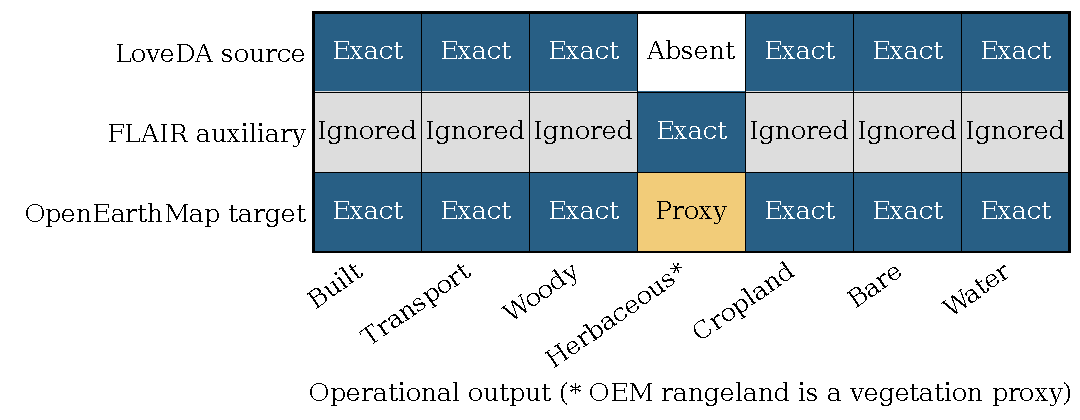
\includegraphics[width=0.92\textwidth]{fig1_coverage_20261015.pdf}
  \caption{Declared operational coverage for the primary source mixture and OpenEarthMap target. Exact means a raw label is mapped to the named common leaf under the fixed crosswalk; it does not assert universal semantic equivalence. LoveDA has no admitted source label for the herbaceous output. B1 retains FLAIR raw ID 10 and ignores all other FLAIR labels. The OEM cell marked Proxy reflects its broader rangeland definition, including shrubs (Supplementary Section S2). Semantic Drone is evaluated separately as grass versus all other pixels (Section~\ref{sec:semanticdrone_result}).}
  \label{fig:coverage}
\end{figure}

\subsection{An auxiliary FLAIR source recovers OpenEarthMap rangeland}
\label{sec:oem_result}

The largest primary contrast is concentrated in the audited missing leaf. Across the three fixed checkpoints, B0 rangeland IoU is $1.6\times10^{-7}$, 0, and 0, whereas B1 reaches 0.3124, 0.3187, and 0.3041 for seeds 19, 37, and 73. The mean paired contrast is +0.3118 with a 95\% evaluation-unit bootstrap interval of [+0.2821, +0.3399] on the Paris-excluded 74-city population (Table~\ref{tab:oem-seeds}, Figure~\ref{fig:oem-primary}). The interval resamples declared city units and is conditional on the completed checkpoints.

\begin{figure}[H]
  \centering
  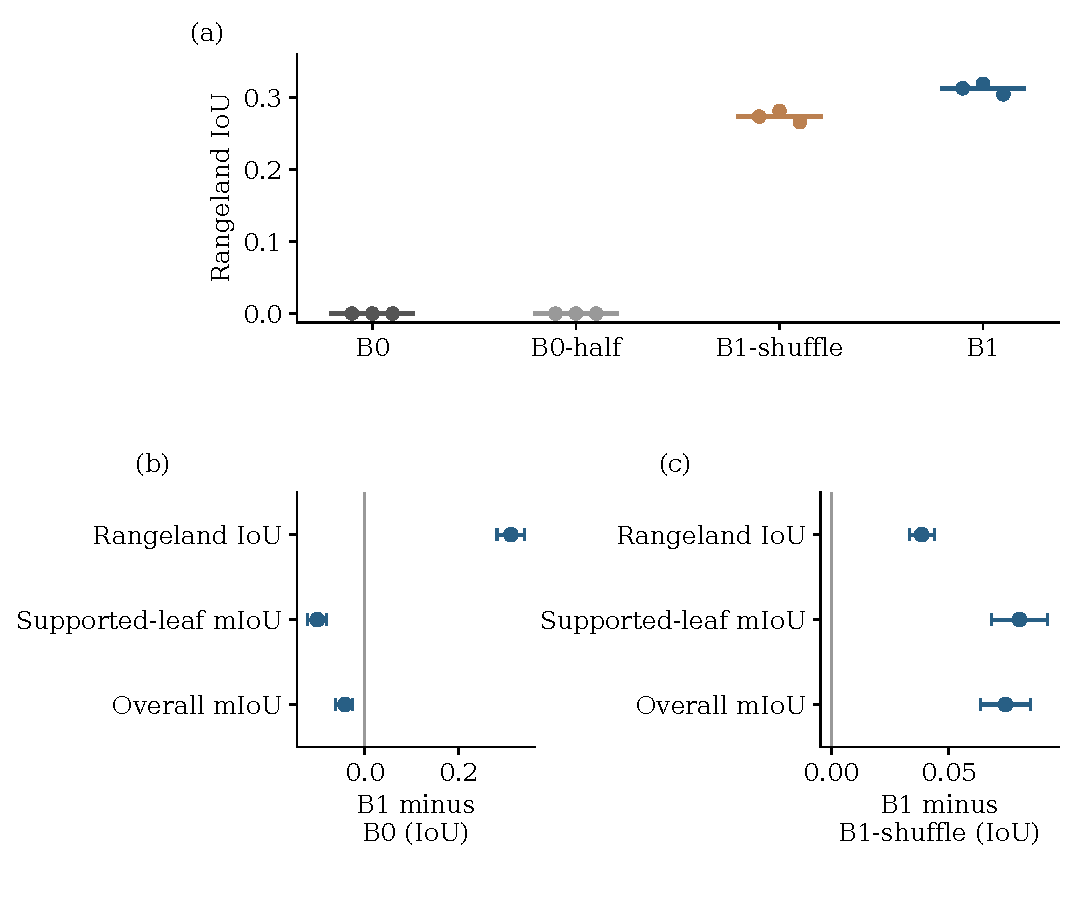
\includegraphics[width=0.92\textwidth]{fig2_oem_results_20261015.pdf}
  \caption{OpenEarthMap results on the Paris-excluded 74-city population. (a) Rangeland IoU for seeds 19, 37 and 73, with horizontal marks showing their mean; horizontal offsets separate checkpoints. (b) B1 minus B0 contrasts. (c) B1 minus the recorded B1-shuffle configuration. Panels (b) and (c) use different axis ranges and show 95\% paired city-bootstrap intervals from 2,000 draws, conditional on the three completed checkpoints. Supported-leaf mIoU averages the six LoveDA-supported leaves. Complete original shuffle schedules were not recovered: panel (c) is a configuration-based sensitivity, not a fully revalidated pairing mechanism.}
  \label{fig:oem-primary}
\end{figure}

Reduced LoveDA exposure alone does not reproduce the observed target-leaf recovery. B0-half lowers overall mIoU by 0.0069 relative to B0, while B1 retains a rangeland gain of +0.3118 after LoveDA exposure is matched (Table~\ref{tab:oem-controls}). The duplicated-crop integrity check is zero at the reported precision and is reported in Appendix Table~\ref{tab:batch_integrity}; it checks the update implementation rather than a generic batch-size effect.

\subsection{Sensitivity to the recorded pairing configuration}
\label{sec:pairing_result}

The archived B1-shuffle configuration specifies the same FLAIR image schedule and mask-density multiset with non-native masks. Full raw schedules were not recovered for independent revalidation of these constraints. It still recovers rangeland, with seedwise IoUs of 0.2732, 0.2812, and 0.2653. Its mean contrast against B0 is 0.2732, compared with 0.3118 for B1--B0. Thus, 0.2732/0.3118 = 87.6\% of the observed recovery remains in this mismatched-pair schedule, and the native B1 configuration is higher by +0.0385 (12.4\%; 95\% evaluation-unit bootstrap interval [+0.0333, +0.0439]); all three seedwise contrasts are positive. The same comparison improves overall mIoU by +0.0741 and mIoU over the six LoveDA-supported leaves by +0.0801 (Table~\ref{tab:oem-controls}). This arithmetic partition describes the specified schedules. It does not separate auxiliary image content from label support, and, because the raw primary schedules are unavailable for independent revalidation, it is reported as a configuration-based sensitivity rather than a fully verified pairing mechanism.

\begin{table}[H]
\centering
\caption{OpenEarthMap Paris-excluded 74-city replay metrics by fixed checkpoint. Values are displayed to four decimal places; the B0 rangeland IoU for seed 19 is $1.6\times10^{-7}$ and those for seeds 37 and 73 are zero. The B0 and B1 supported-leaf mIoU ranges are 0.4359--0.4468 and 0.3309--0.3473, respectively. Supported-leaf mIoU averages the six leaves with exact operational LoveDA support; it is reported beside overall mIoU rather than as an alternative overall-performance estimate. City-bootstrap contrasts are computed from unrounded checkpoint metrics and rounded only for display (Table~\ref{tab:oem-controls}).}
\label{tab:oem-seeds}
\small
\renewcommand{\arraystretch}{1.12}
\setlength{\tabcolsep}{4pt}
\begin{tabular*}{\linewidth}{@{\extracolsep{\fill}}lrrrr@{}}
\toprule
Arm & Seed & Overall mIoU & Rangeland IoU & Supported-leaf mIoU \\
\midrule
B0 & 19 & 0.3830 & 0.0000 & 0.4468 \\
B0 & 37 & 0.3802 & 0.0000 & 0.4436 \\
B0 & 73 & 0.3736 & 0.0000 & 0.4359 \\
B0-half & 19 & 0.3652 & 0.0000 & 0.4261 \\
B0-half & 37 & 0.3825 & 0.0000 & 0.4462 \\
B0-half & 73 & 0.3683 & 0.0000 & 0.4296 \\
B1-shuffle & 19 & 0.2710 & 0.2732 & 0.2707 \\
B1-shuffle & 37 & 0.2564 & 0.2812 & 0.2523 \\
B1-shuffle & 73 & 0.2604 & 0.2653 & 0.2596 \\
B1 & 19 & 0.3400 & 0.3124 & 0.3446 \\
B1 & 37 & 0.3292 & 0.3187 & 0.3309 \\
B1 & 73 & 0.3411 & 0.3041 & 0.3473 \\
\bottomrule
\end{tabular*}
\end{table}

\begin{table}[H]
\centering
\caption{Fixed-budget and shuffled-pairing OpenEarthMap control contrasts on the Paris-excluded 74-city population. Intervals are paired city-bootstrap intervals conditional on completed fixed checkpoints. Contrasts are computed from unrounded checkpoint metrics and rounded only for display. The duplicated-crop integrity check is reported in Appendix Table~\ref{tab:batch_integrity}.}
\label{tab:oem-controls}
\small
\renewcommand{\arraystretch}{1.12}
\setlength{\tabcolsep}{4pt}
\begin{tabular*}{\linewidth}{@{\extracolsep{\fill}}llrrr@{}}
\toprule
Contrast & Metric & Estimate & 95\% lower & 95\% upper \\
\midrule
B0-half $-$ B0 & overall mIoU & $-0.0069$ & $-0.0100$ & $-0.0038$ \\
B1 $-$ B0 & overall mIoU & $-0.0422$ & $-0.0613$ & $-0.0252$ \\
B1 $-$ B0 & rangeland IoU & $+0.3118$ & $+0.2821$ & $+0.3399$ \\
B1 $-$ B0-half & overall mIoU & $-0.0352$ & $-0.0538$ & $-0.0182$ \\
B1 $-$ B0-half & rangeland IoU & $+0.3118$ & $+0.2821$ & $+0.3399$ \\
B1 $-$ B0 & supported-leaf mIoU & $-0.1011$ & $-0.1213$ & $-0.0821$ \\
B1 $-$ B0-half & supported-leaf mIoU & $-0.0931$ & $-0.1128$ & $-0.0741$ \\
B1 $-$ B1-shuffle & overall mIoU & $+0.0741$ & $+0.0634$ & $+0.0848$ \\
B1 $-$ B1-shuffle & supported-leaf mIoU & $+0.0801$ & $+0.0682$ & $+0.0921$ \\
B1 $-$ B1-shuffle & rangeland IoU & $+0.0385$ & $+0.0333$ & $+0.0439$ \\
\bottomrule
\end{tabular*}
\end{table}


\subsection{Recovery is accompanied by a supported-leaf trade-off}
\label{sec:tradeoff_result}

The target-leaf gain does not improve the full operating profile. B1 mean mIoU is 0.3368 compared with 0.3789 for B0, while mIoU over the six leaves with exact operational LoveDA support changes by -0.1011 (95\% evaluation-unit bootstrap interval [-0.1213, -0.0821]). The two metrics answer different questions: overall mIoU includes the recovered rangeland leaf, whereas the defined supported-leaf metric excludes it to report the retained LoveDA leaves. Their numerical differences are therefore not competing effect-size estimates. The seed-level supported-leaf mIoU ranges from 0.4359 to 0.4468 for B0 and from 0.3309 to 0.3473 for B1 (Table~\ref{tab:oem-seeds}); inference remains the declared city-unit bootstrap, not a three-seed test. Matching LoveDA exposure leaves a supported-leaf contrast of -0.0931 for B1--B0-half (Table~\ref{tab:oem-controls}). Figure~\ref{fig:oem-tradeoff} shows the leafwise pattern: rangeland is recovered, whereas the largest observed supported-leaf decline is cropland. Complete unadjusted descriptive intervals are reported in Appendix Table~\ref{tab:all_leaf_contrasts}.

\begin{figure}[H]
  \centering
  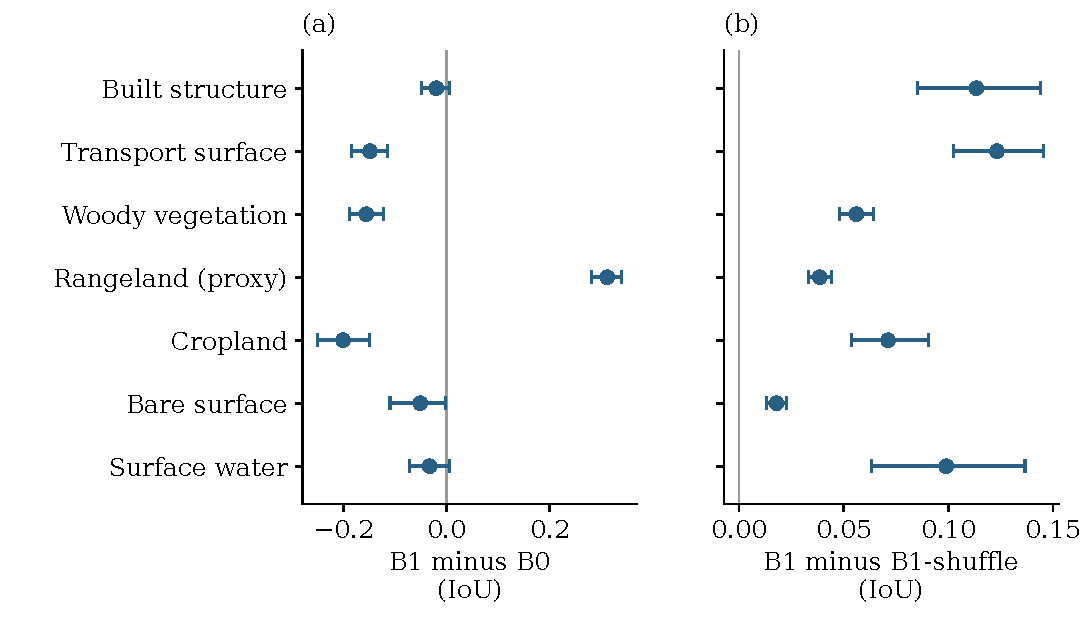
\includegraphics[width=0.92\textwidth]{fig3_leaf_contrasts_20261015.pdf}
  \caption{Leafwise OpenEarthMap contrasts on the Paris-excluded 74-city population. (a) B1 minus B0; (b) B1 minus the recorded B1-shuffle configuration. Both panels use the same seven leaf rows and report 95\% descriptive paired city-bootstrap intervals from 2,000 draws, conditional on checkpoints 19, 37 and 73. Panel (b) is a configuration-based sensitivity: complete original shuffle schedules were not recovered for independent revalidation of pairing and exposure constraints. The two panels use different horizontal scales.}
  \label{fig:oem-tradeoff}
\end{figure}

\subsection{The archived native U-Net comparison repeats the direction}
\label{sec:unet_result}
Across the three archived native U-Net checkpoints, U-B0 and U-B0-half both give zero rangeland IoU. U-B1 gives 0.2957, 0.2767 and 0.2762, with mean 0.2828 and sample SD 0.0111. The U-B1--U-B0 contrast is +0.2828 (95\% checkpoint-conditional paired city interval [+0.2512, +0.3133]). Supported-leaf mIoU changes from 0.2329 to 0.1025, a contrast of -0.1304 (interval [-0.1529, -0.1075]); against U-B0-half it changes by -0.1182 (interval [-0.1390, -0.0965]). Every matched seed has positive rangeland recovery and lower supported-leaf mIoU for both native baseline comparisons (Table~\ref{tab:unet-native}).

The archived evaluation records therefore show recovery with retention loss in a second recorded architecture on the common target. They do not supply an independent target population, a pure-label causal experiment or a CLIP--U-Net superiority comparison. Original checkpoint, spatial reference and historical-code provenance limits remain as specified in Section~\ref{sec:unet_protocol}. Shuffled U-Net results do not enter this conclusion.

\begin{table}[H]
\centering
\caption{Archived native U-Net comparison on the same Paris-excluded 74-city OpenEarthMap target (2,638 rasters). Means and sample SDs summarize the three recorded seed checkpoints; SDs are descriptive. Contrasts use 2,000 paired city draws and 95\% intervals conditional on the fixed recorded checkpoints, not training-seed uncertainty. Supported-leaf mIoU averages the six LoveDA-supported leaves. U-B0-half matches LoveDA exposure in U-B1. Original checkpoint and spatial reference bytes were not replayed; this is a within-family archived-record comparison.}
\label{tab:unet-native}
\small
\setlength{\tabcolsep}{3pt}
\begin{tabular*}{\linewidth}{@{\extracolsep{\fill}}lrrr@{}}
\toprule
Arm & Rangeland IoU & Supported-leaf mIoU & Overall mIoU \\
\midrule
U-B0 & $0.0000 \pm 0.0000$ & $0.2329 \pm 0.0158$ & $0.1996 \pm 0.0136$ \\
U-B0-half & $0.0000 \pm 0.0000$ & $0.2207 \pm 0.0261$ & $0.1892 \pm 0.0223$ \\
U-B1 & $0.2828 \pm 0.0111$ & $0.1025 \pm 0.0209$ & $0.1283 \pm 0.0190$ \\
\bottomrule
\end{tabular*}
\par\medskip
\begin{tabular*}{\linewidth}{@{\extracolsep{\fill}}lrrr@{}}
\toprule
Contrast and metric & Estimate & 95\% lower & 95\% upper \\
\midrule
U-B1 $-$ U-B0 / rangeland & $+0.2828$ & $+0.2512$ & $+0.3133$ \\
U-B1 $-$ U-B0 / supported & $-0.1304$ & $-0.1529$ & $-0.1075$ \\
U-B1 $-$ U-B0-half / rangeland & $+0.2828$ & $+0.2512$ & $+0.3133$ \\
U-B1 $-$ U-B0-half / supported & $-0.1182$ & $-0.1390$ & $-0.0965$ \\
\bottomrule
\end{tabular*}
\end{table}


\subsection{Second target evaluation on Semantic Drone}
\label{sec:semanticdrone_result}

On the primary 400-raster evaluation, frozen E0 gives grass IoU 0.0224, whereas each of the three LoveDA-only B0 checkpoints gives 0.0000. The three B1 checkpoints give 0.2282, 0.2305, and 0.2228 (mean 0.2272; sample SD 0.0040). The descriptive mean B1--B0 contrast is +0.2272 (Supplementary Sections S9 and S11). No three-checkpoint raster-resampling interval is claimed in this revision. The E0-to-B0 decline is a checkpoint diagnostic consistent with LoveDA-only calibration suppressing the limited grass score present in the frozen probe; it does not identify the mechanism. This is a second-target evaluation of the primary source mixture, not a model-level replication: it reuses the probe, prompts, and training budget. The archived record identifies the target manifest and source-archive hashes; independently timestamped pre-inference provenance is not established here.





\subsection{A second source mixture shows the same recovery--trade-off direction}
\label{sec:second_mixture_result}

The source-role-reversed case begins with a different audited gap: Semantic Drone has no exact operational cropland label, whereas LoveDA agriculture and OpenEarthMap \texttt{agriculture\_land} provide declared cropland support. On the frozen 72-city OpenEarthMap population, SD-B0 and the exposure-matched SD-B0-half produce cropland IoU of zero for every seed. SD-B1 reaches 0.1627, 0.1642, and 0.1627, giving a mean paired SD-B1--SD-B0 difference of +0.1632 (95\% evaluation-unit bootstrap interval: [+0.1262, +0.2049]; Table~\ref{tab:second-mixture}).

The recovery again carries a fixed-budget cost. Over the three leaves with exact operational Semantic Drone support, SD-B1 changes base-source mIoU by -0.1686 relative to SD-B0 (95\% evaluation-unit bootstrap interval [-0.1903, -0.1464]) and by -0.1337 relative to exposure-matched SD-B0-half (interval [-0.1534, -0.1151]). The planned shuffled auxiliary-mask arm met multiset and no-native-pair constraints, but its post-run schedule audit found per-pair density mismatches and retired the contrast. Its efficacy is not interpreted. This case tests a second audited source mixture, not a second pairing-control result or an independent target-pair replication.

\begin{table}[H]
\centering
\caption{Second source-mixture replay: Semantic Drone as the base source, LoveDA agriculture as an auxiliary source supplying cropland supervision, and OpenEarthMap as the target. The base-source metric averages the three leaves with exact operational Semantic Drone support: herbaceous vegetation, woody vegetation, and surface water. Point values average three completed checkpoints. Contrasts are computed from unrounded checkpoint metrics and rounded only for display. Intervals are paired 2,000-draw city-bootstrap intervals conditioned on those checkpoints and the 72-city target population excluding Shanghai, Tyrol, and Vienna.}
\label{tab:second-mixture}
\small
\renewcommand{\arraystretch}{1.12}
\setlength{\tabcolsep}{4pt}
\begin{tabular*}{\linewidth}{@{\extracolsep{\fill}}lrrrr@{}}
\toprule
\multicolumn{5}{l}{Cropland IoU by checkpoint and its mean} \\
Arm & Seed 19 & Seed 37 & Seed 73 & Mean \\
\midrule
SD-B0 & 0.0000 & 0.0000 & 0.0000 & 0.0000 \\
SD-B0-half & 0.0000 & 0.0000 & 0.0000 & 0.0000 \\
SD-B1 & 0.1627 & 0.1642 & 0.1627 & 0.1632 \\
\bottomrule
\end{tabular*}
\par\medskip
\begin{tabular*}{\linewidth}{@{\extracolsep{\fill}}lrl@{}}
\toprule
Arm & Base-source mIoU & Role \\
\midrule
SD-B0 & 0.2686 & Base source \\
SD-B0-half & 0.2337 & Exposure control \\
SD-B1 & 0.1001 & Auxiliary cropland source \\
\bottomrule
\end{tabular*}
\par\medskip
\begin{tabular*}{\linewidth}{@{\extracolsep{\fill}}lrrr@{}}
\toprule
SD-B1 minus SD-B0 & Estimate & 95\% lower & 95\% upper \\
\midrule
Cropland IoU & +0.1632 & +0.1262 & +0.2049 \\
Base-source mIoU & -0.1686 & -0.1903 & -0.1464 \\
\bottomrule
\end{tabular*}
\par\smallskip
\raggedright All three checkpoint-specific cropland contrasts are positive.
\end{table}


The separate B2 learnability diagnostic is reported in Supplementary Sections S8 and S11. They do not select or alter the primary source-mixture endpoints.
